\documentclass[aspectratio=169]{beamer}
\usetheme{metropolis}

\usepackage[utf8]{inputenc}
\usepackage[T1]{fontenc}
\usepackage{lmodern}
\usepackage{hyperref}
\metroset{block=fill}
\usepackage{booktabs}
\usepackage{tikz}
\usetikzlibrary{positioning}

\title{Quantum learning pipeline}
\subtitle{Exploring an implementation for Support Vector Machines}
\author{\textbf{Mario Bifulco}, Luca Roversi}
\date{10\textsuperscript{th} September}
\institute{University of Turin}

\begin{document}

\maketitle

\begin{frame}
    \frametitle{Why Quantum Support Vector Machines?}
    
    \begin{alertblock}{Classical SVM limitations}
        \begin{itemize}
            \item Quadratic complexity scaling
            \item Kernel calculation bottlenecks
            \item Hard optimization for high-dimensional data
        \end{itemize}
    \end{alertblock}

    \begin{exampleblock}{Quantum Computing Advantage}
        \begin{itemize}
            \item Quantum parallelism for kernel calculation
            \item Quantum tunneling to escape local minima 
        \end{itemize}
    \end{exampleblock}

\end{frame}

\begin{frame}
    \frametitle{What is a Quantum Support Vector Machine?}

    \begin{block}{Gate-based approach}
        \begin{enumerate}
            \item Encoding classical data via quantum feature map
            \item Estimate kernel via quantum circuit evaluation
            \item Classical SVM training with quantum kernel
        \end{enumerate}
    \end{block}

    \begin{block}{Annealing-based approach}
        \begin{itemize}
            \item Classical kernel calculation
            \item SVM optimization problem reduction to QUBO formulation
            \item SVM training via quantum annealing
        \end{itemize}
    \end{block}

\end{frame}

\begin{frame}
    \frametitle{Quantum kernels}

    \begin{enumerate}
        \item Raw input encoding
        \item PCA to retain $N$ most significant features (8, 16, 30)
        \item Encoding with a feature map (\texttt{Z}, \texttt{ZZ}, \texttt{SU2HR}, \texttt{SU2RR}) repeated $k$ times (1, 2, 3)
        \item Compute kernel as $|\langle\phi(x_i)|\phi(x_j)\rangle|^2$
    \end{enumerate}

    \begin{figure}
        \includegraphics[height=0.45\textheight]{su2hr4qubit2rep.png}
    \end{figure}

\end{frame}

\begin{frame}
    \frametitle{Finding a good quantum kernel}

    \begin{table}
        \begin{tabular}{cccc}
            \toprule
            \textbf{\# Qubits} & \textbf{Feature Map} & \textbf{Repetitions} & \textbf{Alignment (KTA)} \\
            \midrule
            30                 & SU2HR                & 1                    & 98.650\%                 \\
            8                  & ZMAP                 & 2                    & 93.558\%                 \\
            16                 & SU2RR                & 1                    & 91.203\%                 \\
            \bottomrule
        \end{tabular}
    \end{table}

\end{frame}

\begin{frame}
    \frametitle{Quantum annealing SVM}

    \begin{columns}
        \begin{column}{0.5\textwidth}
            \begin{figure}
                \begin{center}
                    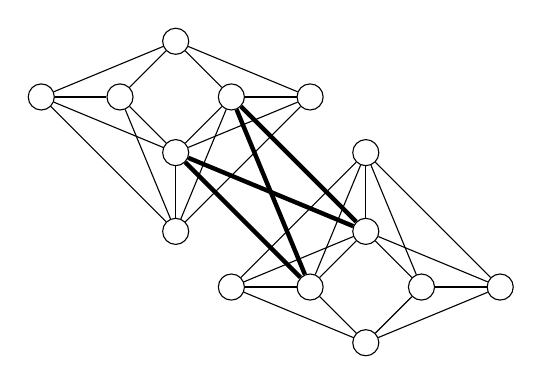
\begin{tikzpicture}[main/.style = {draw, circle}] 
                        \node[main](1){};
                        \node[main](2)[right of=1]{}; 
                        \node[main](5)[above right of=2]{};
                        \node[main](3)[below right of=5]{};
                        \node[main](4)[right of=3]{};
                        \node[main](7)[below right of=2]{};
                        \node[main](8)[below of=7]{};
                
                        \draw (4) -- (8);\draw (8) -- (1);\draw (2) -- (8);\draw (8) -- (3);
                        \draw (1) -- (5);\draw (5) -- (4);\draw (4) -- (7);\draw (7) -- (1);
                        \draw (2) -- (5);\draw (5) -- (3);\draw (3) -- (7);\draw (7) -- (2);
                        \draw (1) -- (2);\draw (4) -- (3);\draw (8) -- (7);
                
                        \node[main](11)[below right of=4]{};
                        \node[main](12)[below of=11]{};
                        \node[main](13)[below left of=12]{};
                        \node[main](14)[left of=13]{};
                        \node[main](15)[below right of=13]{};
                        \node[main](16)[below right of=12]{};
                        \node[main](18)[right of=16]{};
                
                        \draw (11) -- (12);\draw (11) -- (13);\draw (11) -- (14);\draw (11) -- (16); 
                        \draw (12) -- (13);\draw (12) -- (16);\draw (15) -- (13);\draw (15) -- (16);
                        \draw (11) -- (18);\draw (14) -- (13);\draw (14) -- (15);\draw (18) -- (15);
                        \draw (18) -- (16);\draw (12) -- (14);\draw (12) -- (18);

                        \draw[ultra thick] (3) -- (12);
                        \draw[ultra thick] (3) -- (13);
                        \draw[ultra thick] (7) -- (12);
                        \draw[ultra thick] (7) -- (13);
                    \end{tikzpicture} 
                    \caption{16 qubit QPU}
                \end{center}
            \end{figure}
        \end{column}
        \begin{column}{0.5\textwidth}
            \begin{figure}
                \begin{center}
                    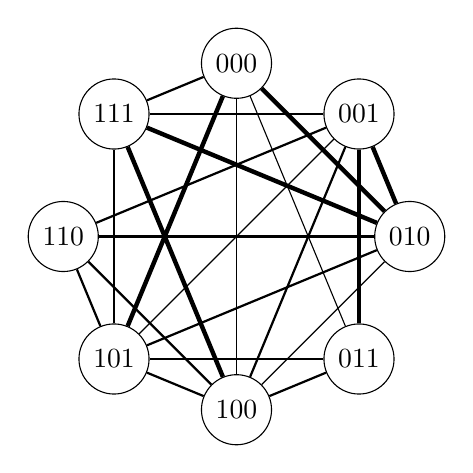
\begin{tikzpicture}[main/.style = {draw, circle}] 
                        \node[main] (n0) at (90:2.2cm)  {000};
                        \node[main] (n1) at (45:2.2cm)  {001};
                        \node[main] (n2) at (0:2.2cm)   {010};
                        \node[main] (n3) at (315:2.2cm) {011};
                        \node[main] (n4) at (270:2.2cm) {100};
                        \node[main] (n5) at (225:2.2cm) {101};
                        \node[main] (n6) at (180:2.2cm) {110};
                        \node[main] (n7) at (135:2.2cm) {111};

                        \draw [ultra thick] (n0) -- (n2);
                        \draw (n0) -- (n3);
                        \draw (n0) -- (n4);
                        \draw [ultra thick] (n0) -- (n5);
                        \draw [thick] (n0) -- (n7);
                        \draw [ultra thick] (n1) -- (n2);
                        \draw [ultra thick] (n1) -- (n3);
                        \draw [thick] (n1) -- (n4);
                        \draw (n1) -- (n5);
                        \draw [thick] (n1) -- (n6);
                        \draw (n1) -- (n7);
                        \draw (n2) -- (n4);
                        \draw [thick] (n2) -- (n5);
                        \draw [thick] (n2) -- (n6);
                        \draw [ultra thick] (n2) -- (n7);
                        \draw [thick] (n3) -- (n4);
                        \draw (n3) -- (n5);
                        \draw [thick] (n4) -- (n5);
                        \draw [thick] (n4) -- (n6);
                        \draw [ultra thick] (n4) -- (n7);
                        \draw [thick] (n5) -- (n6);
                        \draw [thick] (n5) -- (n7);
                    \end{tikzpicture} 
                    \caption{States of a 3 bit problem}
                \end{center}
            \end{figure}
        \end{column}
    \end{columns}

\end{frame}

\begin{frame}
    \frametitle{Choosing an appropriate regularization parameter}

    \begin{alertblock}{Problem}
        SVM requires a fixed regularization parameter ($C$)

        This parameter must be represented in binary format
    \end{alertblock}

    \begin{exampleblock}{Solution}
        Set the upper bound of $C$ to $2^n-1$ to minimize the number of unused bits
    \end{exampleblock}

\end{frame}

\begin{frame}
    \frametitle{Fully quantum pipeline}

    \begin{alertblock}{Training}
        \begin{enumerate}
            \item \textbf{Gate-based kernel calculation}
            \item \emph{Kernel matrix export}
            \item \textbf{Annealing-based optimization}
        \end{enumerate}
    \end{alertblock}
    
    \begin{block}{Output}
        A model ready for classical inference
    \end{block}

\end{frame}

\begin{frame}
    \frametitle{Results}

    \begin{block}{Main findings}
        We achieved an \texttt{F1-score} of 90\%
        \begin{itemize}
            \item 30 qubit kernel
            \item an upper bound of 255 for the regularization parameter
        \end{itemize}

        This model performs comparably to a classical SVM with an RBF kernel
    \end{block}

    \begin{alertblock}{Future works}
        \begin{itemize}
            \item Improved preprocessing pipeline
            \item Comprehensive analysis of the impact of kernel dimensionality
        \end{itemize}
    \end{alertblock}

\end{frame}

\begin{frame}
    \frametitle{Thanks for your attention!}

    \begin{columns}
        \begin{column}{0.5\textwidth}
            \centering
            \begin{figure}
                \includegraphics[height=0.6\textheight]{repo.png}
            \end{figure}
            Access the code and read the full paper
        \end{column}
        \begin{column}{0.5\textwidth}
            For further questions, feel free to contact me (\texttt{mario.bifulco@unito.it})
        \end{column}
    \end{columns}

\end{frame}

\end{document}